% Number 770
% CoEM  CopM Algebra Units Vectors
% Ballistic pendulum - usual, ETM conceptual argument
% JG

% Watermark
\AddToShipoutPicture*{\BackgroundPic}

\addtocounter {ProbNum} {1}

%\begin{floatingfigure}[r]{.44\textwidth}
%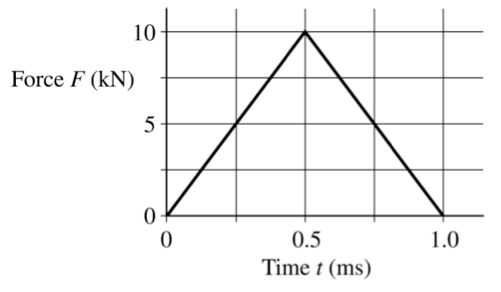
\includegraphics[scale=.5]{/Users/jgates/desktop/latex/pics/collisiongraph1}
%\end{floatingfigure}
 
{\bf \Large{\arabic{ProbNum}}} A 30 g bullet is shot into a 2.5 kg block of wood that is hanging from an 80 cm long rope. The bullet embeds itself in the wood, and the wood's suqsequent motion causes the rope to reach a maximum angle of 46 degrees from the vertical.\bigskip

Determine the initial speed of the bullet. \paragraph{}
\noindent
\vfill

As the block swings back towards its initial position, consider the moment when the rope is inclined 15 degrees from the vertical.  

\bigskip
What is the speed of the block at this moment? Compare the total energy of the bullet/block/Earth system at this moment and at the moment just before the bullet struck the block.  Explain the reason for the difference.
\vfill

Use the directions of the forces acting on the block at this moment and the direction of its motion to make an energy-based argument about why the block speeds up more quickly at this moment than it will when it is closer to its starting point.
\vfill
%\hfill 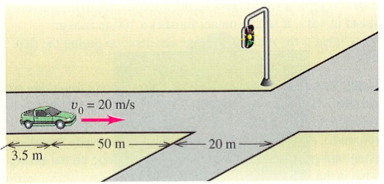
\includegraphics[scale=.85]{/Users/jgates/desktop/latex/pics/redlight.png}
\newpage